% This file was created by tikzplotlib v0.9.8.
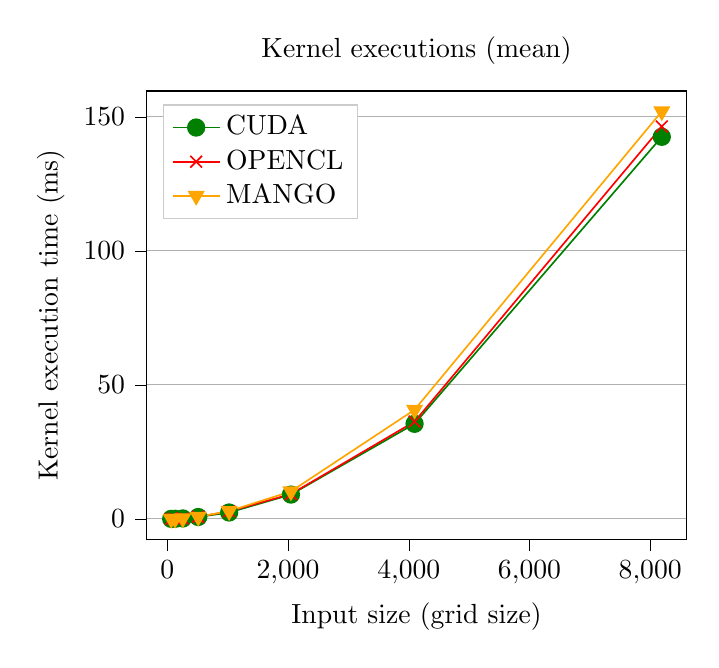
\begin{tikzpicture}

\definecolor{color0}{rgb}{1,0.647058823529412,0}

\begin{axis}[
legend cell align={left},
legend style={
  fill opacity=1,
  draw opacity=1,
  text opacity=1,
  at={(0.03,0.97)},
  anchor=north west,
  draw=white!80!black
},
tick align=outside,
tick pos=left,
title={Kernel executions (mean)},
x grid style={white!69.0196078431373!black},
xlabel={Input size (grid size)},
xmin=-342.4, xmax=8598.4,
xtick style={color=black},
y grid style={white!69.0196078431373!black},
ylabel={Kernel execution time (ms)},
ymajorgrids,
ymin=-7.58184667491691, ymax=159.663488779392,
ytick style={color=black}
]
\addplot [semithick, green!50.1960784313725!black, mark=*, mark size=3, mark options={solid}]
table {%
64 0.0202140275516594
128 0.0516223956466069
256 0.184729111111111
512 0.725393121412804
1024 2.39956375632911
2048 9.09626238291139
4096 35.4947399367089
8192 142.560531045161
};
\addlegendentry{CUDA}
\addplot [semithick, red, mark=x, mark size=3, mark options={solid}]
table {%
64 0.0204119285237141
128 0.0538414779706275
256 0.190541695364238
512 0.780070042826552
1024 2.83085394321767
2048 9.27893204444444
4096 36.3103518152866
8192 146.39821255625
};
\addlegendentry{OPENCL}
\addplot [semithick, color0, mark=triangle*, mark size=3, mark options={solid,rotate=180}]
table {%
64 0.0414139624681934
128 0.0703628888888889
256 0.211658812903226
512 0.81808229004329
1024 2.9290935968254
2048 10.27900955
4096 40.7308336708861
8192 152.061428076923
};
\addlegendentry{MANGO}
\end{axis}

\end{tikzpicture}
